\section{Stationary processes}

\begin{definition}[\textit{Strongly stationary process}]
    A process is called strongly stationary if:
    \[F_{t_1,t_2,\dots,t_n}(\dots)=F_{t_1+\tau,t_2+\tau,\dots,t_n+\tau}(\dots)\]
\end{definition}

\begin{definition}[\textit{Weakly stationary process}]
    A process is called weakly stationary if both the mean and the covariance are stationary:
    \[\begin{cases}
        \mu(t)=\mu(t+\tau) \qquad \forall \tau \\
        \gamma(t_1,t_2)=\gamma(t_1+\tau,t_2+\tau) \qquad \forall \tau
    \end{cases}\]
\end{definition}
The first condition ensures that the value of $\mu(t)$ remains constant, while the second condition ensures that $\gamma(\tau)$, where $\tau=t_2-t_1$, remains constant.
\begin{example}
    Consider the experiment of flipping a coin. 
    The outcome of the experiment can be either heads or tails. 
    This can be viewed as the combination of two processes:
    \[v_{head}(t)=\sin\left(\dfrac{2 \pi t}{N}\right) \qquad v_{tail}(t)=-\sin\left(\dfrac{2 \pi t}{N}\right)\]
    \begin{figure}[H]
        \centering
        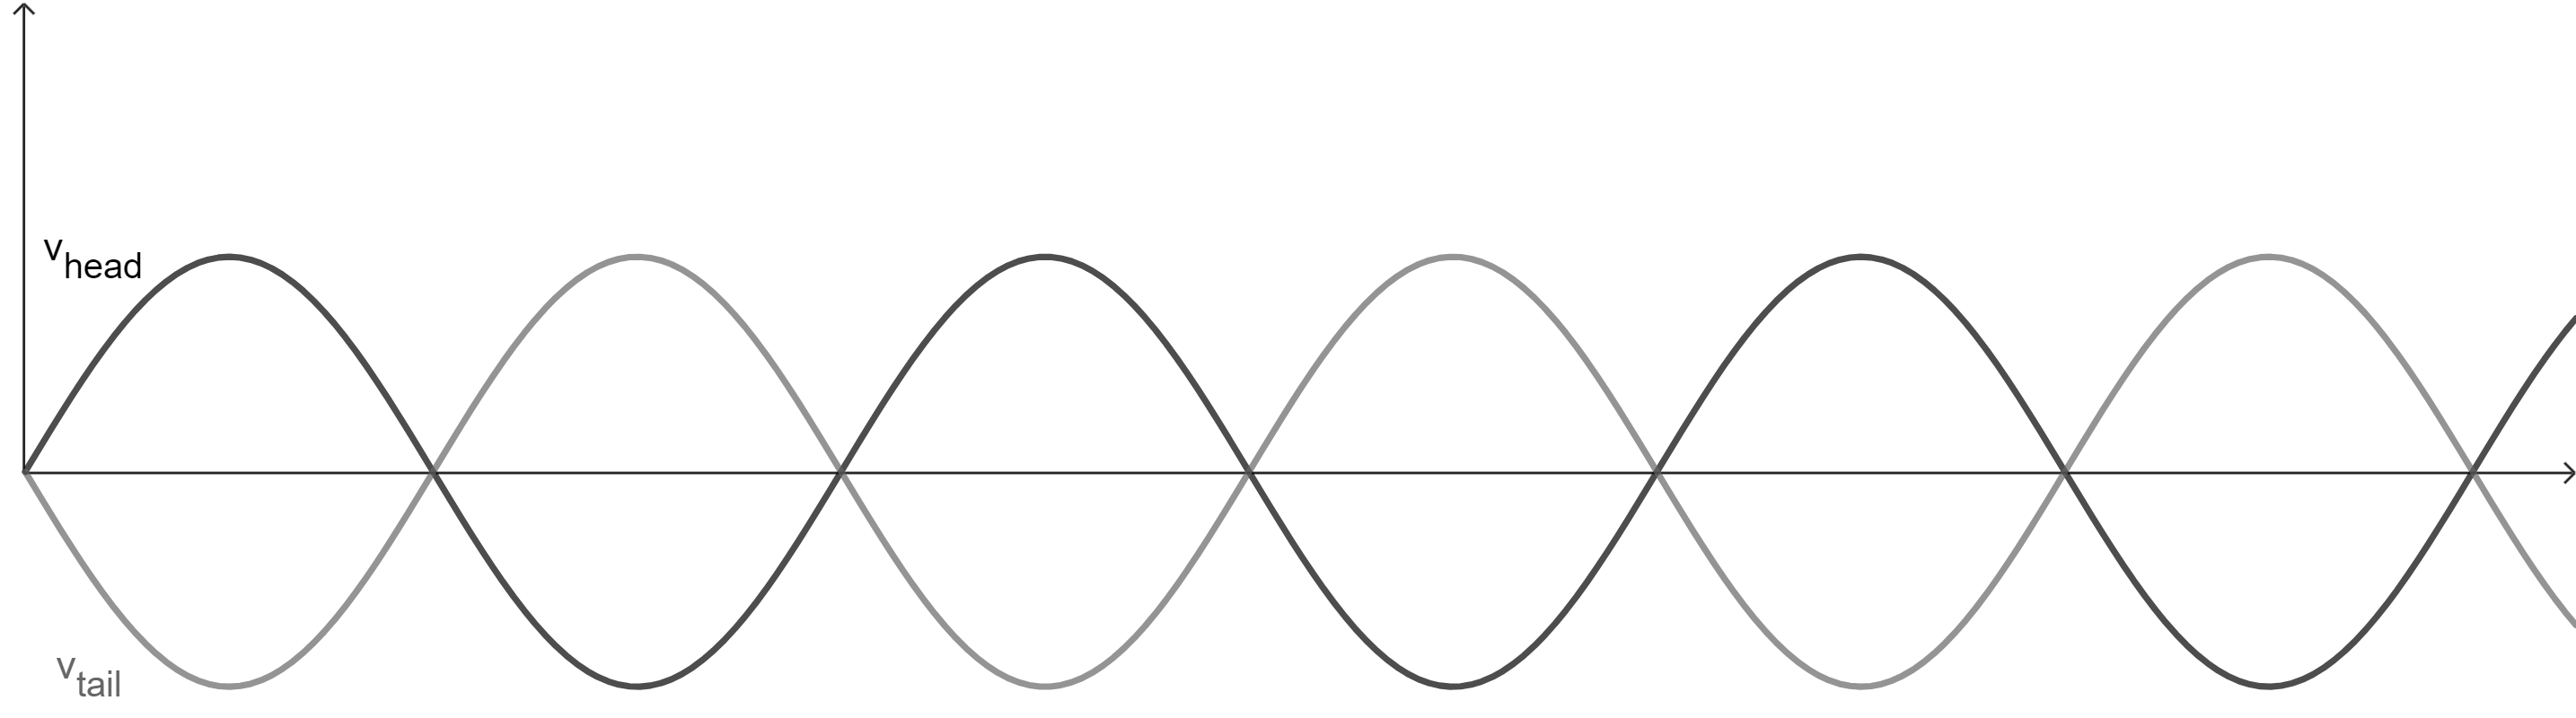
\includegraphics[width=0.75\linewidth]{images/tailhead.png}
        \caption{Graphs of the functions $v_{head}(t)$ and $v_{tail}(t)$}
    \end{figure}
    The expected mean $\mu(t)$ is zero for each time instant, making it constant.
    However, the variance is zero only when both functions intersect the $t$-axis, and it is greater than zero at all other instances.
    Consequently, the variance is not constant, indicating that the process is not stationary.
\end{example}
\newpage
\begin{example}
    Consider the process $v(t)=\bar{v}$, where $\bar{v} \sim G(1,3)$. 
    \begin{figure}[H]
        \centering
        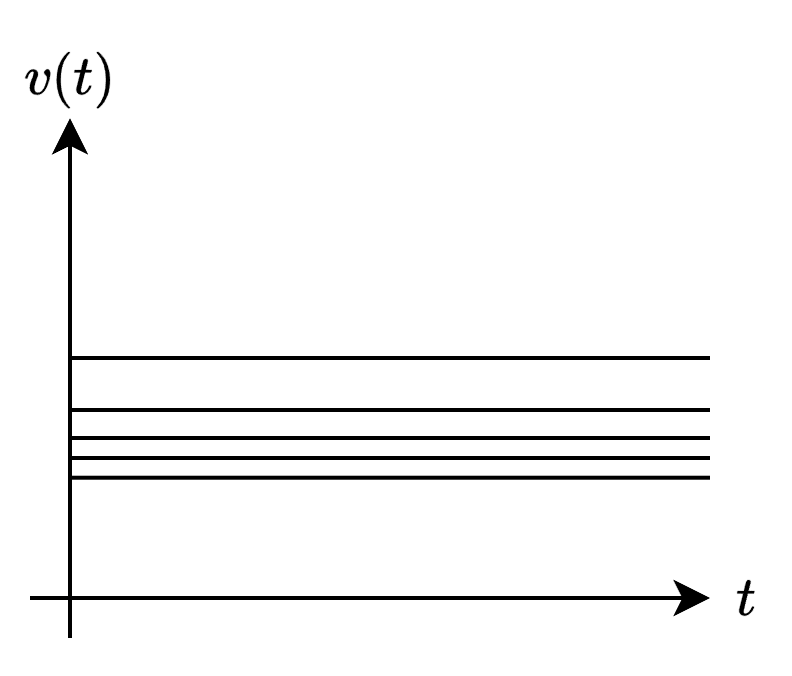
\includegraphics[width=0.25\linewidth]{images/static.png}
        \caption{Some possible realizations}
    \end{figure}
    We have that: 
    \[\mu(t)=\mathbb{E}\left[v(t)\right]=\mathbb{E}\left[\bar{v}\right]=1\]
    Thus, the expected mean value is constant.

    For the covariance, we have: 
    \begin{align*}
        \gamma(t,t+\tau)&=\mathbb{E}\left[\left(v(t)-1\right)\left(v(t+\tau)-1\right)\right] \\
                        &=\mathbb{E}\left[\left(\bar{v}-1\right)\left(\bar{v}-1\right)\right] \\
                        &=\mathbb{E}\left[\left(\bar{v}-1\right)^2\right] \\
                        &=\text{Var}\left[\bar{v}\right] \\
                        &=3
    \end{align*}
    Furthermore, the $\gamma$ function is constant, indicating that the process is weakly stationary.
\end{example}
\begin{example}
    Consider the process $v(t)=t\bar{v}-t$, where $\bar{v} \sim G(1,3)$. 
    \begin{figure}[H]
        \centering
        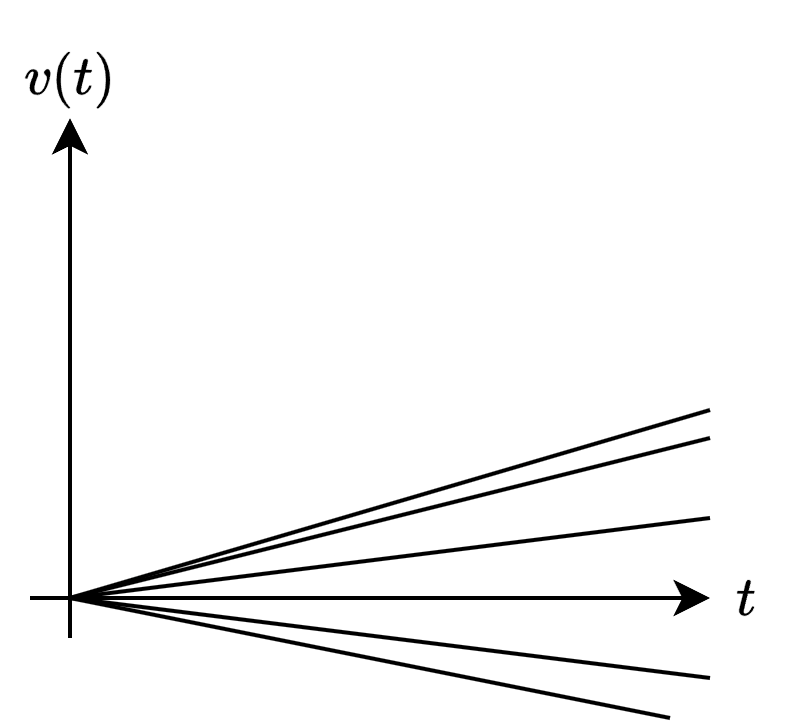
\includegraphics[width=0.25\linewidth]{images/stationary.png}
        \caption{Some possible realizations}
    \end{figure}
    We have:
    \[\mu(t)=\mathbb{E}\left[v(t)\right]=\mathbb{E}\left[t\bar{v}-t\right]=t\mathbb{E}\left[\bar{v}\right]-t=t\cdot 1-t=0\]
    Thus, the expected mean value is constant.

    For the covariance, we have:
    \begin{align*}
        \gamma(t,t+\tau)&=\mathbb{E}\left[\left(v(t)-1\right)\left(v(t+\tau)-1\right)\right] \\
                        &=\mathbb{E}\left[\left(t\bar{v}-t-0\right)\left(\left(t+\tau\right)\bar{v}-\left(t+\tau\right)-0\right)\right] \\
                        &=\mathbb{E}\left[t\left(\bar{v}-1\right)\left(t+\tau\right)\left(\bar{v}-1\right)\right] \\
                        &=t\left(t+\tau\right)\mathbb{E}\left[\left(\bar{v}-1\right)^2\right] \\
                        &=3t\left(t+\tau\right)
    \end{align*}
    Since the $\gamma$ function is not constant, the process is not stationary.
\end{example}

\subsection{Properties of weakly stationary stochastic processes}
For a weakly stationary stochastic process, the following properties hold:
\begin{itemize}
    \item $\mathbb{E}\left[ v(t) \right]=\mu$ 
    \item $\gamma(\tau)=\mathbb{E}\left[ (v(t)-\mu)(v(t+\tau)-\mu) \right]$
    \item $\tilde{\gamma}=\mathbb{E}\left[v(t)v(t+\tau)\right]$
\end{itemize}
These properties exhibit the following characteristics:
\begin{itemize}
    \item $\gamma(0)=\mathbb{E}\left[\left(v(t)-\mu\right)^2\right]=\text{Var}\left[v(t)\right]$
    \item $\left\lvert \gamma(\tau) \right\rvert \leq \gamma(0) \qquad \forall\tau$
    \item $\gamma(\tau)=\gamma(-\tau)$ (even function). 
    \item The Toepliz matrix:
        \[\begin{bmatrix}
            \gamma(0)   & \gamma(1)     & \gamma(2)     & \dots     & \gamma(N-1)   \\
            \gamma(1)   & \gamma(0)     & \gamma(1)     & \dots     & \gamma(N-2)   \\
            \gamma(2)   & \gamma(1)     & \gamma(0)     & \dots     & \gamma(N-3)   \\
            \vdots      & \vdots        & \vdots        & \vdots    & \vdots        \\
            \gamma(N-1) & \gamma(N-2)   & \gamma(N-3)   & \dots     & \gamma(0)     \\
        \end{bmatrix}\]
        is a semi-definite matrix, requiring its determinant to be greater than or equal to zero.
\end{itemize}

\subsection{Gaussian processes}
A Gaussian process is defined by the property that its probability distribution function follows a joint Gaussian distribution:
\[F_{t_1,t_2,\dots,t_n}(\dots)=\dfrac{1}{\sigma\sqrt{2\pi}}e^{-\frac{1}{2}\left(\frac{t-\mu}{\sigma}\right)^2}\]
\begin{property}
    If a Gaussian process is weakly stationary, it implies that it is also strongly stationary.
\end{property}

\subsection{Ergodic processes}
In an ergodic process, the statistical properties can be accurately derived from the analysis of a single realization, with a probability approaching one as the number of observations tends to infinity:
\[\lim_{N \rightarrow \infty}\dfrac{1}{N}\sum_{i=1}^N\cdot = \mathbb{E}\left[\cdot\right]\]